\newcommand{\MyTitle}{Cricket Scenario}
\documentclass[a5paper,10pt]{article}

\usepackage[utf8]{inputenc}
\usepackage[swedish]{babel}
\usepackage[T1]{fontenc}
\usepackage[pdftex]{graphicx}
\usepackage{calc,xparse,geometry}
\usepackage{wrapfig}
\usepackage[pagestyles]{titlesec}

\graphicspath{ {./../Bilder/} }
\newpagestyle{mine}{%
\sethead[\thepage][{\raisebox{\dimexpr\headheight + \topmargin + \voffset + 1in-0.75in\relax}[0pt][0pt]{
\includegraphics[width = .75\textwidth]{horn}}}][]
{}{{\raisebox{\dimexpr\headheight + \topmargin + \voffset + 1in-0.75in\relax}[0pt][0pt]{
\includegraphics[width = .75\textwidth]{horn}}}}{\thepage}
\setfoot{}{}{}
}
\pagestyle{mine}
\author{Gustav Ruthgård}
\title{\MyTitle}
\date{\today}

\usepackage{xkeyval}

\makeatletter
\define@cmdkey{rpg}[char@]{name}[]{}
\define@cmdkey{rpg}[char@]{class}[]{}
\define@cmdkey{rpg}[char@]{kropp}[]{}
\define@cmdkey{rpg}[char@]{reaktion}[]{}
\define@cmdkey{rpg}[char@]{sinne}[]{}
\define@cmdkey{rpg}[char@]{special}[]{}
\define@cmdkey{rpg}[char@]{width}[\linewidth]{}

\define@cmdkey{move}[char@]{rubrik}[]{}
\define@cmdkey{move}[char@]{beskrivning}[]{}
\define@cmdkey{move}[char@]{grundegenskap}[]{}
\define@cmdkey{move}[char@]{lyckat}[]{}
\define@cmdkey{move}[char@]{mitten}[]{}
\define@cmdkey{move}[char@]{misslyckat}[]{}
\define@cmdkey{move}[char@]{val}[]{}
\define@cmdkey{move}[char@]{width}[\linewidth]{}

\define@cmdkey{scenen}[char@]{typ}[]{}
\define@cmdkey{scenen}[char@]{namn}[]{}
\define@cmdkey{scenen}[char@]{rubrik}[]{}
\define@cmdkey{scenen}[char@]{plats}[]{}
\define@cmdkey{scenen}[char@]{birollett}[]{}
\define@cmdkey{scenen}[char@]{birolltva}[]{}
\define@cmdkey{scenen}[char@]{birolltre}[]{}
\define@cmdkey{scenen}[char@]{width}[\linewidth]{}

\newcommand{\statlabel}{\textsc}

\usepackage{calc,xparse}
\newlength\mycardwidth
\setlength\mycardwidth{.75\textwidth}
\NewDocumentCommand \boxme { O{} }{%
  \fbox{%
    \parbox{\linewidth-2\fboxrule-2.5\fboxsep}{\strut #1}%
  }%
}
\NewDocumentCommand \pageme { O{} O{} }{%
  \begin{minipage}{#1\mycardwidth}
    \centering\boxme[#2]
  \end{minipage}%
}
\NewDocumentCommand \cardme { O{.75\textwidth} +m }{%
  \setlength\mycardwidth{#1-2\fboxrule-2\fboxsep}%
  \fbox{%
    \begin{minipage}{\mycardwidth}
      \centering
      #2%
    \end{minipage}%
  }%
}

\newcommand{\setcharacterstats}[1]{%
  \begingroup
  \setkeys{rpg}{name,class,kropp,reaktion,sinne,special,width,#1}%
  \noindent
  \cardme[\textwidth]{%
    \pageme[.69][\statlabel{Namn}: \char@name]%
    \pageme[.31][\statlabel{\char@class}]

    \pageme[.33][\statlabel{Kropp}: \char@kropp]%
    \pageme[.34][\statlabel{Reaktion}: \char@reaktion]%
    \pageme[.33][\statlabel{Sinne}: \char@sinne]
    \raggedright \textit{S�tt ut +2, +1, 0}

    \pageme[][\statlabel{Specialdrag}:]
    \raggedright \textit{\char@special}
  }
}
\newcommand{\displaymove}[1]{%
  \begingroup
  \setkeys{move}{rubrik,beskrivning,grundegenskap,lyckat,mitten,misslyckat,val,width,#1}%
  \noindent
  \cardme[\textwidth]{%
    \pageme[.69][\statlabel{\char@rubrik}]%
    \pageme[.31][\statlabel{Sl�} +\char@grundegenskap]

    \pageme[.99][\char@beskrivning]

    \pageme[.31][\statlabel{10+}]%
    \pageme[.69][\char@lyckat]

    \pageme[.31][\statlabel{7-9}]%
    \pageme[.69][\char@mitten]

    \pageme[.31][\statlabel{2-6}]%
    \pageme[.69][\char@misslyckat]

    \pageme[.99][\char@val]%
  }
}
\newcommand{\satscen}[1]{%
  \begingroup
  \setkeys{scenen}{typ,namn,rubrik,plats,birollett,birolltva,birolltre,width,#1}%
  \noindent
  \cardme[\textwidth]{%
    \pageme[1][\statlabel{\textbf{\char@typ}}]

    \pageme[1][\statlabel{Rubrik:} \char@rubrik]

    \pageme[.31][\statlabel{Huvudroll:} \char@namn]%
    \pageme[.69][\statlabel{Plats:} \char@plats]

    \pageme[1][\statlabel{Plats:} \char@plats]

    \pageme[.33][\statlabel{Biroll: } \char@birollett]%
    \pageme[.34][\statlabel{Biroll: } \char@birolltva]%
    \pageme[.33][\statlabel{Biroll: } \char@birolltre]
  }
}
\newcommand{\rollformular}[1]{%
  \begingroup
  \setkeys{rpg}{name,class,kropp,reaktion,sinne,special,width,#1}%
  \noindent
  \cardme[\textwidth]{%
    \pageme[.69][\statlabel{Namn}: \char@name]%
    \pageme[.31][\statlabel{Koncept}:]
    \pageme[][\statlabel{R�dsla}:]
    \pageme[][\statlabel{Drivkraft}:]

    \pageme[.33][\statlabel{Kropp}: \char@kropp]%
    \pageme[.34][\statlabel{Reaktion}: \char@reaktion]%
    \pageme[.33][\statlabel{Sinne}: \char@sinne]
    \pageme[][\statlabel{Specialdrag}:]
  }
}
\makeatletter

\begin{document}
\maketitle
%\clearpage
%\clearpage
\part{Spelardrag}
Din rollperson kan utf�ra alla dessa drag som en f�ljd av att du agerar p� olika s�tt i en scen. N�r du s�ger vad din rollperson g�r kan SL d� be dig sl� f�r ett av dessa drag.
\section{Attakera}
\textit{N�r du attackerar n�gon som k�mpar tillbaka v�lj hur}

och sl�r \textbf{+Kropp}
\begin{itemize}
  \item[10+] Du lyckas och undviker motst�ndarens attack.
  \item[7-9] Du attackerar motst�ndaren men till ett pris. Spelledaren v�ljer 1:
  \begin{itemize}
    \item Du tr�ffas av ett motanfall.
    \item Du g�r mindre skada.
    \item Du f�rlorar n�got.
    \item Du g�r av med all ammo.
    \item Du uts�tts f�r ett nytt hot.
    \item Du f�r senare problem.
  \end{itemize}
  \item[2-6] SL g�r ett mjukt eller h�rt drag.
\end{itemize}
\clearpage
\section{Undvika}
\textit{N�r du undviker, blockerar eller parerar skada} sl� \textbf{+Kropp}.
\begin{itemize}
  \item[10+] Du klarar dig helt oskadd.
  \item[7-9] Du klarar dig undan det v�rsta av skadan men spelledaren v�ljer om du hamnar i ett d�ligt l�ge, f�rlorar n�got eller om du inte helt undviker skada.
  \item[2-6] Du reagerar f�r l�ngsamt eller g�r en felbed�mning: kanske undviker du inte alls eller s� hamnar du i ett v�rre l�ge �n du b�rjade i. SL g�r ett drag.
\end{itemize}
\section{Tar skada}
\textit{N�r du uts�tts f�r skada} sl� \textbf{+Kropp}. Har du skydd l�gger du till v�rdet till slaget.
\begin{itemize}
  \item[10+] Du biter ihop och kan forts�tta som vanligt.
  \item[7-9] Du st�r fortfarande p� benen men spelledaren v�ljer:
  \begin{itemize}
    \item Skadan f�r dig att hamna ur balans
    \item Du tappar n�got
    \item Du f�r ett \textbf{allvarligt s�r}
  \end{itemize}
  \item[2-6] Skadan �r �verv�ldigande. Du v�ljer om du:
  \begin{itemize}
    \item �r utslagen f�r resten av scenen(SL avg�r om du �ven f�r ett \textbf{allvarligt s�r}).
    \item F�r ett \textbf{kritisk s�r} men �r vid medvetande (har du redan ett kritiskt s�r kan du inte v�lja detta alternativ igen).
    \item D�r.
  \end{itemize}
\end{itemize}
\subsection{Allvarligt s�r}
S�ret beh�ver n�gon typ av v�rd eller tid f�r att l�ka men blir inte v�rre av sig sj�lvt. Alkohol och sm�rtstillande droger kan ta bort avdraget som s�ret ger om s� bara tillf�lligt.
\subsection{Kritiskt s�r}
S�ret kommer inte l�ka av sig sj�lv utan f�rv�rras. Den som �r kritisk s�rad m�ste ha v�rd inom kort f�r att inte d�.
\subsection{Avdrag fr�n s�r}
Om du har icke-stabiliserade allvarliga och/eller kritiska s�r drabbas du av avdrag, enligt nedan.
Om du har
\begin{itemize}
  \item ...minst ett allvarligt s�r; -1 Kropp
  \item ...ett kritiskt s�r; -1 Kropp
  \item ...b�de minst ett allvarlig s�r och ett kritiskt s�r; -2 Kropp
\end{itemize}
Om du dricker alkohol, tar sm�rtstillande, eller bed�var din sm�rta p� liknande s�tt, neutraliserar du avdraget fr�n dina \textbf{allvarliga s�r} under en kortare tidsperiod, vanligen under en scen. Detta g�ller inte kritiska s�r.
\clearpage
\section{�verblicka}
\textit{N�r du �verblickar situationen} sl� \textbf{+Reaktion}. Vid lyckat kan du st�lla fr�gor till spelledaren. N�r du agerar p� spelledarens r�d ta +1 p� ditt slag.
\begin{itemize}
  \item[10+] St�ll 2 fr�gor.
  \item[7-9] St�ll 1 fr�ga.
  \item[2-6] Du f�r st�lla en fr�ga �nd� men du drar till dig o�nskad uppm�rksamhet eller uts�tter dig f�r fara.
\end{itemize}
Fr�gor
\begin{itemize}
  \item Vad �r min b�sta v�g f�rbi hindret?
  \item Vad �r det st�rsta hotet mot mig?
  \item Vad kan jag anv�nda till min f�rdel?
  \item Vad beh�ver jag vara vaksam p�?
  \item Finns det n�got g�mt h�r?
  \item �r det n�got som �r underligt?
\end{itemize}
\section{L�sa av en person}
\textit{N�r du l�ser av en person} sl� \textbf{+Reaktion}
\begin{itemize}
  \item[10+] St�ll 2 fr�gor.
  \item[7-9] St�ll 1 fr�ga.
  \item[2-6] Du f�r st�lla en fr�ga �nd� men du drar till dig o�nskad uppm�rksamhet eller uts�tter dig f�r fara.
\end{itemize}
Medan du talar med personen du l�ser av kan du spendera dina fr�gor 1 f�r 1 f�r att st�lla deras spelare/spelledaren fr�gor:
\begin{itemize}
  \item Ljuger du?
  \item Vad k�nner du just nu?
  \item Vad t�nker du g�ra?
  \item Vad �nskar du att jag g�r?
  \item Hur kan jag f� dig att ... ?
  \item �r det n�got som �r underligt?
\end{itemize}
\section{Unders�ka}
\textit{N�r du unders�ker n�gonting}, sl� \textbf{+Sinne}. Om du lyckas s� finner du alla direkta ledtr�dar och f�r st�lla fr�gor f�r att f� mera information.
\begin{itemize}
  \item[10+] Fr�ga tv� fr�gor
  \item[7-9] Fr�ga en fr�ga, men svaret kostar dig n�got. SL best�mmer vad; du beh�ver n�gon eller n�got f�r att f�rst� svaret, eller det tar dig extra tid att f� reda p� svaret.
  \item[2-6] Du f�r fr�ga en fr�ga �nd�, men du uts�tts f�r ov�ntad fara eller annan kostnad.
\end{itemize}
Fr�gor:
\begin{itemize}
 \item Hur kan jag f� reda p� mer om vad jag unders�ker?
 \item Vad s�ger min magk�nsla om vad jag unders�ker?
 \item �r det n�got konstigt med det jag unders�ker?
\end{itemize}
\section{�vertala}
\textit{N�r du �vertalar en spelledarperson genom f�rhandling, argumentation eller utifr�n en maktposition} sl� \textbf{+Sinne}.
\begin{itemize}
  \item[10+] Hon ger vika.
  \item[7-9] Hon g�r som du vill men (SL v�ljer):
  \begin{itemize}
    \item Hon �r inte n�jd och ber om mer i geng�ld.
    \item �vertalningen skapar problem vid ett senare tillf�lle.
    \item Hon ger med sig men �r os�ker (�vertalningens effekt �r bara tillf�llig).
  \end{itemize}
  \item[2-6] �vertalningsf�rs�ket har oavsiktliga konsekvenser. SL g�r ett drag.
\end{itemize}

\textit{N�r du f�rs�ker �vertala en rollperson} sl� \textbf{+Sinne}.
\begin{itemize}
  \item[10+] Rollpersonen v�ljer sj�lv om hon ger med sig eller inte, du ger dock b�da effekterna nedan.
  \item[7-9] Rollpersonen v�ljer sj�lv om hon ger med sig eller inte, du v�ljer dock en effekt nedan.
  \item[2-6] Rollpersonen �r fri att g�ra som hon vill och har +1 p� n�sta slag mot dig. Ingen av effekterna nedan g�ller.
\end{itemize}
Effekter:
\begin{itemize}
  \item Hon motiveras att g�ra som du vill (hon f�r +1 p� n�sta slag).
  \item Hon drabbas av tvivel om hon inte g�r som du vill (hon f�r -1 V�lm�ende).
\end{itemize}
\section{Agera under hot}
\textit{N�r du g�r n�got riskabelt, �r under tidspress eller f�rs�ker undkomma fara, ber�ttar SL vad hotet �r}, sl� \textbf{+Sinne} f�r att agera trotts hotet.
\begin{itemize}
  \item[10+] Du g�r det.
  \item[7-9] Du g�r det, men tvekar, blir f�rdr�jd, eller m�ste reagera p� en komplikation - SL ger dig ett ov�ntat resultat, ett h�gt pris eller ett sv�rt val.
  \item[2-6] Det blir konsekvenser, du g�r misstag eller s� uts�tts du f�r fara. SL g�r ett mjukt eller h�rt drag.
\end{itemize}
\section{Sj�lvkontroll}
\textit{N�r du anv�nder din sj�lvkontroll f�r att st� emot psykisk p�verkan eller p�frestning som stress, traumatiska upplevelser och �vernaturliga krafter} sl� \textbf{+Sinne}
\begin{itemize}
  \item[10+] Du biter ihop och kan forts�tta op�verkad.
  \item[7-9] Du st�r emot men anstr�ngningen ger dig ett tillst�nd som varar tills du f�tt tillf�lle att �terh�mta dig. V�lj en:
  \begin{itemize}
    \item Du blir arg, ledsen, r�dd eller skuldtyngd. (-1 V�lm�ende).
    \item Du blir h�nf�rd (+1 Relation till det som orsakar tillst�ndet).
    \item Du blir distraherad (-2 i situationer d�r tillst�ndet begr�nsar dig).
    \item Du hems�ks av upplevelsen senare (SL f�r en h�llhake).
  \end{itemize}
  \item[2-6] Du f�rlorar kontrollen och SL v�ljer mellan att du �r maktl�s inf�r hotet, panikslagen utan kontroll �ver dina handlingar eller  m�r d�ligt av traumat (s�nk V�lm�ende enligt traumats styrka).
  \begin{itemize}
    \item Allvarligt trauma (-2 V�lm�ende)
    \item Livsavg�rande trauma (-4 V�lm�ende)
  \end{itemize}
\end{itemize}
\section{V�lm�ende}
V�lm�ende �r ett m�tt p� hur pass balanserat rollpersonens psyke �r. En rollperson �r till en b�rjan kontrollerad men kan sjunka i V�lm�ende n�r hon �r med om traumatiska upplevelser.
\begin{table}[!h]
\begin{tabular}{|c| l l|}
\hline & Kontrollerad & \\
\hline & Olustig & \textbf{Lindrig stress:} \\
& Ofokuserad &  \textit{-1 Sinne} \\
\hline & Skakad &  \textbf{Allvarlig stress:} \\
& Stressad & \textit{-1 Sj�lvkontroll, -2 Sinne} \\
& Neurotisk &  \\
\hline & �ngestdrabbad &  \textbf{Kritisk stress:} \\
 & Irrationell &  \textit{-2 Sj�lvkontroll, -3 Sinne} \\
 & Okontrollerad &  \\
\hline & Nedbruten & Spelledaren g�r ett drag \\
\hline
\end{tabular}
\end{table}
\section{Hj�lpa eller motarbeta}
\textit{N�r du hj�lper eller motarbetar en annan rollperson}, sl� och l�gg till ditt attribut f�r samma drag som den andra rollperson sl�r f�r.
\begin{itemize}
  \item[10+] Ge rollpersonen +2 eller -2 p� slaget.
  \item[7-9] Ge rollpersonen +1 eller -1 p� slaget.
  \item[2-6] N�got g�r fel f�r dig. SL g�r ett drag.
\end{itemize}


\clearpage
\part{Bakgrund}
\section{Timelocks}
Tidslås skapas genom att sätta upp enormt kraftfulla Timeflux enheter. Dessa enheter existerar i alla fyra dimensioner och är så kraftfulla att de inte går att förgöra förens deras kraftkällor börjar sina. Tidslåsen gör det näst intill omöjligt att resa tillbaka till den perioden. Ända sättet att manipulera tiden under ett tidslås är att helt enkelt bara ha en fungerande organisation som lever vanliga liv utan tidsresande.
\section{Agentaktiviteter under tidslåsen}
Det första stora tidskriget som pågått i 192 år avslutades 1502 när Leonardo Da Vinci offrade sitt liv för att etablera en enormt kraftull Timefluxenhet. Tidsresor in i tidskrigets slut blev väldigt frekventa och många justeringar genomfördes för att få in så många agenter som möjligt i olika hemliga sälskap. Illuminati, tempelherreorden och många andra slutna sällskap blev grogrunden för dessa agenter. De skapade skrifter om vad deras efterkommande skulle leta efter för tecken och hur de skulle bygga upp organisationen för att hålla människorna i skack.
\subsection{Rebellerna - Människorna}
Efter att Leonardo avslutat tidsresorna fanns inte många upplysta kvar vilket ledde till att enbart några få som avslöjat någon av agenternas riktiga agendor eller avhoppare från dessa känner till vad som egentligen "finns där ute". Förberedelserna inför tidslåsets upphörande blev därför få. Under 1980-talet är de mest tin foil hats. Och liknande nördar som ingen tror på.
\subsection{Cyprox incorperate - Förgörarna}
I det stora kriget föll Cyprox som de stora förlorarna då de förintats och deras sändpunkter i framtiden avslöjats för Ginnies. Några enstaka celler överlevde och enbart en mindre organisation lyckades hålla fast greppet genom tidens tand. Under 1980 talet finns de enbart kvar i nordkorea förklädda till den statens ledare.
\subsection{Ginnies - Avledarna}
Ginnies blev de stora vinnarna dels på grund av deras kamp mot Cyprox från den sändande epok där kriget mellan parterna också pågår. Ginnies slår sig i allians med Rebellerna och deras ledare Leonardo under slutet av 1480-talet och lyckas på så sätt till slut ta över. Efter att låset kommer på plats har deras tidsarkitekter kommit dit och dirigerar hårt vad som skall hända framåt. De sår sina frön utifrån den kunskap de besitter och lyckas väl med att etablera sig. De har fortfarande stor eller mycket stor maktposition under 1980 talet i form av olika celler runt om i världen. Deras största fästen är i Indien och i USA.
\part{1986 året för återkomsten}
\section{Marylain}
I framtiden sätts nya baser upp för tidsresor och probes skickas tillbaka med hundra års mellanrum, sedan 10 år och slutligen hittar man att vissa probes kommer igenom under början på 1986. Den första agenten kommer fram den 7'e februari. En liten ort i södra USA, Marylain kommer att bli dessa trevande försöks viktigaste plats. Då tidslåset fortfarande gör det mycket svårt att komma fram innan det är avstängt gör att enbart en handfull av resande kommer fram. Alla som når fram har olika uppdrag.
\section{Cyprox}
Cyprox är helt fel ute och tror att Ginnies sin vana trogen etablerar sig i Indien. De hamnar där och bygger sin cell i New Deli. Det tar dem ett antal år att hitta Ginnies agenter vilket gör att deras närvaro i USA är okänd under lång tid.
\section{Ginnies 1986}
Ginnies anländer i byn med två arkitekt en man, Tony Diego och en kvinna Ilena Garsia, och en hacker Jonathan Mercy. De två arkitekterna börjar genast genomföra de förändringar som skall leda fram till att tidslåset faller vid rätt tid. Tony tar anställning i skolan och påbörjar där att värva barn för att få bäst spridning på deras uppdrag. Utvalda elever \textit{vaccineras} och får the cricket gene inplaneterad i sig. De kommer att plockas ca 30 år senare för att vervas in som agenter. Ilena börjar istället på IRS kontoret och gifter sig snart för att få barn.
\subsection{Agenda}
Att börja tippa händelserna mot att tidslåset bryts 2018 så som de vet att det kan göra. För att nå dit behöver de se till att många nog från den lilla orten får möjligheten att utveckla en potent gen. Rätt personer skall sedan identifieras och rekryteras som agenter.
\subsection{Hotet}
\begin{itemize}
  \item[Låg] Arkitekterna börjar bygga upp sina epoker. De etablerar generna och planerar för vilka aktiviteter som behöver komma på plats.
  \item[1:a växeln] Mass spridning av generna genomförs. Utvalda klasser i skolan \textit{vaccineras} för att få genen. Epokerna börjar rullas ut.
  \item[2:a växeln] De vaccinerade börjar följas upp för att identifiera vilka det är. Tidiga tecken på vad som händer de påverkade boxas in.
  \item[3:e växeln] De identifierade familjerna infiltreras och barnen vervas som agenter i tidig ålder.
  \item[Overdrive] Blir de påkomna med allt för hårda bevis undanröjs bevismaterial och vitnen utan pardon.
\end{itemize}
\subsection{Roller}
\subsubsection{Tony Diego}
\textbf{Roll: Arkitekt}\\
\textbf{Drifkraft:} Att sätta upp förutsättningar för att tidslåset skall falla 2018. Tar anställning vid skolan och börjar påverka barnen för att de skall genomdriva hans agenda i framtiden.
\subsubsection{Ilena Garsia}
\bild{namn=Ilena-Garsia,sida=l}
\textbf{Roll: Arkitekt}\\
Drifkraft: Att sätta upp förutsättningar för att tidslåset skall falla 2018. Tar anställning vid sjukhuset och börjar påverka patienter och organisationen för att genomdriva agenda i framtiden.
\subsubsection{Jonathan Mercy}
\bild{namn=Ginne-agent,sida=r}
\textbf{Roll: Hacker}\\
Drivkraft: Skaffa många barn som möjligt för att sprida en genen via blodet vilket ger bästa potensen. Tar anställning på IRS kontoret och börjar där bygga upp och koda om system för att förbereda för återkomsten.
\subsection{Platser}
\subsubsection{Marylain elementary high}
En traditionell highschool där de flesta av stadens ungdomar går. Skolan är byggd i två våningar med en stor ljusgård i mitten. Klassrummen ligger ut efter fasadens kanter och ljusgården är byggd i grå granit med balkonger runt om på andra våningen. Utanför huvudbyggnaden finns en asfalterad plan med basketplan och två större flyglar. Den ena flygeln inrymmer sjukstugan där \textit{Tony Diego} jobbar som Skolsyster.
\subsubsection{Saint Lucys hospital}
Saint Lucys hospital är ett litet sjukhus som ligger i hjärtat av Marylain. Sjukhuset har hög standard och kombinerar privat vård med den basala som finns för de som inte har råd med sjukförsäkringen. I sina mingröna och mintblå uniformer går personalen runt här. Ordningen är mycket god och patienterna är över lag väldigt nöjda med den vård som bedrivs. Sjukhusets ledning styrs av Ginnies och deras vänner. Här administreras och tas gene-sprutorna fram. Det hela görs som ett forskningsprojekt för ny diabetesmedicin, något som får stora medel varje år från privata givare. Genom att gå igenom bokföringen och kanske även genom att ha koll på hur forskningsområdet kring diabetes bedrivs finns en liten chans att man hittar att något fuffens är på gång.
\subsubsection{Lagerhus 13}
Ett av lagerhusen nere i hamnen har byggts om till kontor och hideout för Ginnie agenterna. Lagerhuset ligger i en del av hamnen som tidigare användes som fiskehamn men nu är övergiven. Denna plats används enbart i nödfall och har ett kassaskåp där hemliga dokument och planer finns lagrade. Dokumenten är skrivna på Silomitriksa och bör vara mycket svåra för spelarna att förstå ifall de skulle komma över dem då det språket börjar talas om 3000 år. Vissa ord kan kännas igen om någon är språkforskare på morderna indiska språk.
\subsubsection{IRS kontoret}
IRS sysslar med skattekontroller på både privatpersoner och företag. Här finns naturligt en massa register över befolkningen, hur de flyttar, vart de jobbar och så vidare. Det här är den perfekta platsen för våra arkitekter att övervaka och även planera och genomdriva sina sociala akrikteturer. På kontoret i Marylain jobbar Jonathan Mercy så snart han får chansen att ordna papper osv. Han kommer också att hjälpa andra som kommer resande med att etablera en trovärdig pappersexistens i den här tiden. Kontoret i Marylain är inte så stort, här arbetar ett 20 tal personer och det är ett litet kontor som är utlokaliserat och täcker in en större region än själva Marylain. Lokalen har traditionella kontor och är över lag ganska sunkigt med renovering senast på 60-talet.
\section{Rebeller 1986}
\subsection{Agenda}
I den lilla orten finns ett antal rednecks, en av dem, Ian Parker såg när Tony kom fram genom tidshoppet och är mycket mistänksam, han har också kontaktats av en avhoppare från Ginnie cellen på orten, en annan kille med alkoholproblem som heter Ben Mathews.
\subsection{Hotet}
\begin{itemize}
  \item[Normal] Rednecks do what rednecks does.
  \item[Låg] Då Ian berättar för Ben vad han sett så inser Ben vad som är på gång. Han börjar berätta om de uråldriga sägnerna om tidsresenärerna.
  \item[1:a växeln] Ian och Ben börjar försöka värva andra till sitt cause.
  \item[2:a växeln] Rebellerna har nu fått med ytterligare 3-4 stycken och de börjar sprida rykten om Tony.
  \item[3:e växeln] Rebellerna börjar hota Tony och söker även efter fler tidresenärer. Alla som beter sig konstigt är skyldiga.
  \item[Overdrive] Rebellerna har fått nog och nu skall Tony och de andra dö!
\end{itemize}
\subsection{Roller}
\subsubsection{Ian Parker}
\bild{namn=Rebel,sida=l}
Ian Parker såg när Tony kom fram genom tidshoppet och är mycket mistänksam, han har också kontaktats av en avhoppare från Ginnie cellen på orten, en annan kille med alkoholproblem som heter Ben Mathews.
\subsubsection{Ben Mathews}
\bild{namn=Rebel2,sida=r}
Avhoppare från Ginnies cell i Marylain. Alkoholproblem och desperat. Blir kompis med Ian Parker och inser att det är allvar när Ian berättar att han sett Francis tidshoppa in i nutiden.
\subsection{Platser}
\subsubsection{Stanlies bar and grill}
En klassisk amerikansk bar. Drivs av Tony Tomahawk, en indian som är väldigt råbarkad. Han är vän med Ian trotts att Ian kanske inte alltid har det mest högtravande språket när det kommer till Tony. Stället är kanske inte det mest välbesökta av hela byn, men det har en hel rad stammissar som kommer dit både då och då. Stället har ett gömt rum under ett av förrådsrummen där Tony samlat på sig vapen för en hel pluton rednecks. Tonyt ställer upp och delar ut vapen till behövande rednecks om så krävs för att försvara sig mot skumma tillresta.
\subsubsection{Ians Mobile home}
Maryland outback camping park är ett ställe som var tänkt att locka tursiter till träskområdet där de skulle kunna ställa upp sina fina trailers och ha barbeque partyn på kvällarna. Det slog aldrig igenom och är efter år utan underhåll väldigt slitet och sunkigt. Här står några gamla trailers uppställda som inte tar sig iväg från parken då de inte längre går att köra. Ian bor i en av dessa trailers. Dessutom finns här ett 10 tal andra boenden. Att bo här är högst osäkert då ingen riktigt bryr sig om folk som bor här ute. De kvinnor som sökt sig hit i despiration att få tak över huvudet har ofta fått påhälsning av sina ex-män och blivit både slagna och våldtagna.
\subsection{Bakgrundsscener 1986}
\subsubsection{Ginnies}
\satscen{
  typ = Spelledarscen,
  rubrik = När A's fick sitt agentuppdrag av sin faster innan hon försvann.,
  namn = A: ,
  plats = Hemma hos A's fasters coola funkisvilla.,
  birollett = A's Mamma,
  birolltva = A's Pappa,
  birolltre = A's Farbror
}
\satscen{
  typ = Spelledarscen,
  rubrik = När vi gjorde oss redo för skolresan till Frankrike,
  namn = B:,
  plats = I väntrummet utanför skolsysterns rum,
  birollett = B's Mamma,
  birolltva = Skolsyster,
  birolltre = B's bästa kompis SLP!!!
}
\subsubsection{Rebellerna}
\satscen{
  typ = Spelledarscen,
  rubrik = När farsan sköt Old Tom,
  namn = C:,
  plats = I pappas trailer en regnig höstdag,
  birollett = Old Tom,
  birolltva = Cs pappa Ian Parker,
  birolltre = Ians fru Carol
}
\clearpage
\part{2018 året då tidslåset låses upp}
\section{Scenariots startpunkt}
Arkitekterna har nu förberett allt, det som behövs nu är några tillräckligt mäktiga människor som kan klara av att stänga ned tidslåset. Att göra det kräver en stark gennärvaro och resursfulla personer. Våra arkitekter har sett till att de utvalda är motiverade att komma tillbaka till Marylain för att starta igång med arbetet. De är inte initierade i varför men var och en kommer få ett frö i sin bakgrund som gör att triggern arkitekterna använder sig av görs extra verksam för dem.
\section{Ledtrådskarta}
På följande sätt är ledtrådarna i scenariot ihopkopplade.\\
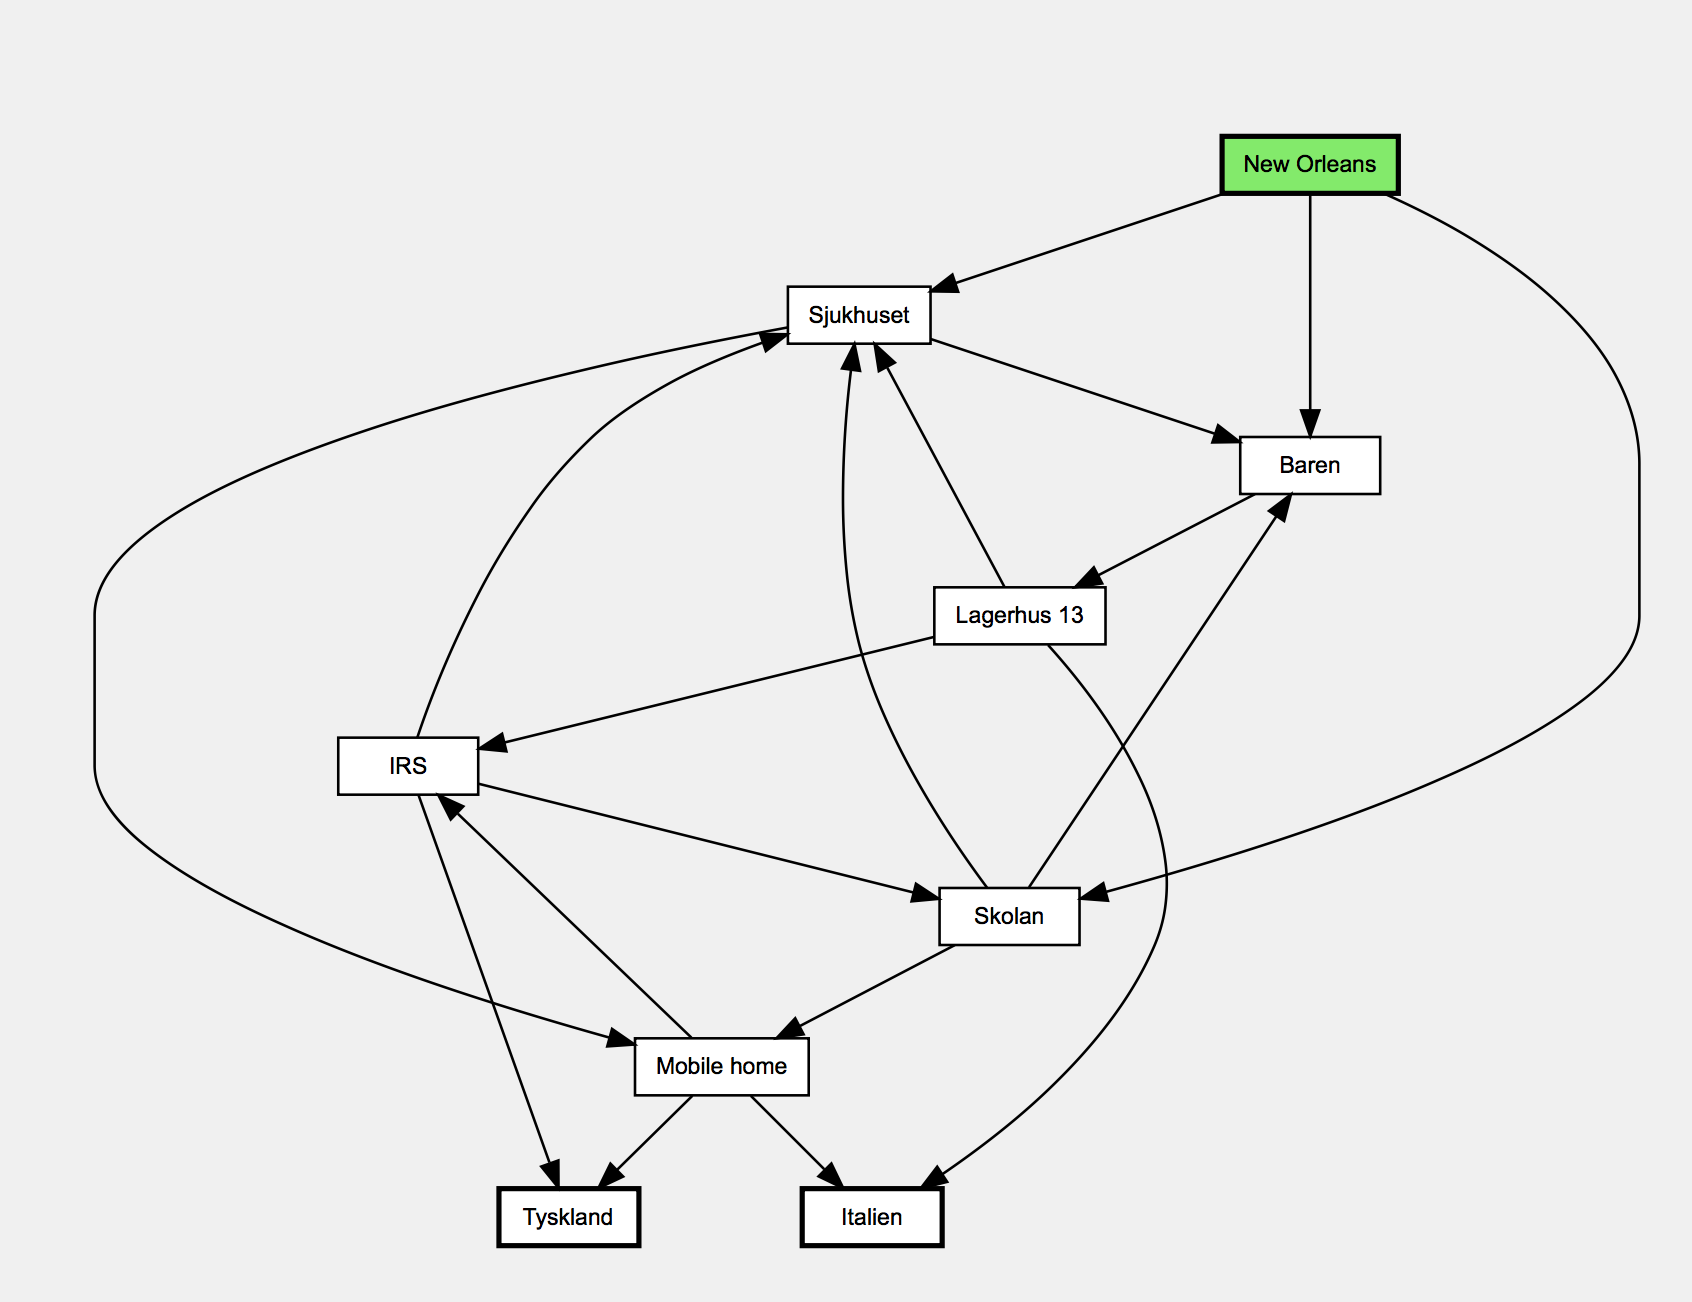
\includegraphics[width=0.9\textwidth]{Cluemap}
\subsection{New Orleans, klassfesten}
Alla rollpersoner befinner sig förmodligen i New Orleans dit de flyttat efter att de blivit vuxna. Rollpersonerna kommer alla att delta i en reunionfest för de som bor i New Orleans eller de som har haft möjligheten att resa dit. En av rollpersonerna får vara den som har bjudit in till träffen och får beskriva vart festen hålls, hur den är planerad osv. Alla rollpersoner får beskriva varför de är där och hur de känner inför att återförenas med sina gamla klasskamrater från Marylain high. Då rollersonerna inte har träffats på typ 20 år så är detta ett utmärkt tillfälle att pressentera sig för varndra om vad man nu för tiden gör i livet mm.
Ledtråd till Sjukhuset
Ledtråd till Baren
Ledtråd till Skolan
\subsection{Sjukhuset}
Ledtråd till Baren
Ledtråd till Mobile home
Ledtråd till Lagerhus 13
\subsection{Baren}
Ledtråd till Skolan
Ledtråd till IRS
\subsection{Skolan}
Ledtråd till Baren
Ledtråd till Sjukhuset
Ledtråd till Lagerhus 13
\subsection{Lagerhus 13}
Ledtråd till Italien
Ledtråd till IRS
\subsection{IRS}
\subsection{Mobile home}
\subsection{Italien}
\subsection{Tyskland}

\subsection{Den mystiska dagboken}

\subsection{Agenda}
agendan
\subsection{Hotet}
hotet
\subsection{Roller}
roll
\subsection{Platser}
plats
\subsection{Växlar}
\begin{itemize}
  \item[Normal] normala
  \item[Låg] låg
  \item[1:a växeln] 1
  \item[2:a växeln] 2
  \item[3:e växeln] 3
  \item[Overdrive] extremt
\end{itemize}

\section{Rebeller 1986}
vilka
\subsection{Agenda}
agendan
\subsection{Hotet}
hotet
\subsection{Roller}
roll
\subsection{Platser}
plats
\subsection{Växlar}
\begin{itemize}
  \item[Normal] normala
  \item[Låg] låg
  \item[1:a växeln] 1
  \item[2:a växeln] 2
  \item[3:e växeln] 3
  \item[Overdrive] extremt
\end{itemize}
\section{Ginnies 2018}
vilka
\subsection{Agenda}
agendan
\subsection{Hotet}
hotet
\subsection{Roller}
roll
\subsection{Platser}
plats
\subsection{Växlar}
\begin{itemize}
  \item[Normal] normala
  \item[Låg] låg
  \item[1:a växeln] 1
  \item[2:a växeln] 2
  \item[3:e växeln] 3
  \item[Overdrive] extremt
\end{itemize}

\section{Rebeller 2018}
vilka
\subsection{Agenda}
agendan
\subsection{Hotet}
hotet
\subsection{Roller}
roll
\subsection{Platser}
plats
\subsection{Växlar}
\begin{itemize}
  \item[Normal] normala
  \item[Låg] låg
  \item[1:a växeln] 1
  \item[2:a växeln] 2
  \item[3:e växeln] 3
  \item[Overdrive] extremt
\end{itemize}


\clearpage
\section{Gamla noteringar}

Ett karaktärspel där karaktärernas bakgrunder knyts in i scenariot. Spelstilen kommer vara starkt narativt driven och reglerna kommer baseras på Kult: Divinity lost men inte världen.

Det första scenariot kommer vara lite deckaraktigt där karaktärerna blir personligt indragna i mystiska försvinnanden.

Karaktärerna har i sin bakgrund varit med om försvinnanden i sin närhet men de har inte varit personliga utan de har helt enkelt bevittnat dessa, men när de var så pass unga att de inte blev trodda.

Ta fram en scen per karaktär där någon i deras omgivning försvinner spårlöst.

I början av scenariot så spelas en scen där någon närstående till karaktären försvinner spårlöst.



Agentscen där en agent rekryterar dem?

Kan agenten vara en av spelarna?

Uppdraget är att hjälpa dem reda ut vem som får folk att försvinna.

Hemliga uppdraget är att skydda dem från att bli tagna.

Hemresan till hemorten?

Platser att hitta med ledtrådar

Biblioteket/Skolbibblan
  Vad har hänt här egntligen? Vad hände när försvinnanden genomfördes? Vilken information skall leda till Ginnies?

Ginnie safe house
  Hur är det skyddat? Vilken verksamhet är dess front?

Timeflux maskinen
  Tungt bevakad
  Utan avstängningsfunktion

Turn off in all dimensions?
  Sight of the aliens?

Liten ort från början, alla har någon som försvinner. Flyttar därifrån på 90 talet, nu när det händer igen så ger ni er tillbaka.

Scen: Lektion i skolan, lärarinnan Asta berättar om Sveriges floder. Plötsligt försvinner hon mitt i en mening. Vad gör klassen.


\end{document}
